\documentclass[a4paper,12pt]{article}
\voffset=-1.5cm
\oddsidemargin=0.0cm
\textwidth = 480pt
\usepackage{eurosym}
\usepackage{vmargin}
\usepackage{amsmath}
\usepackage{graphics}
\usepackage{epsfig}
\usepackage{subfigure}
\usepackage{fancyhdr}
%\usepackage{listings}
\usepackage{amsmath}
\usepackage{graphicx}
\usepackage{amssymb}
\usepackage{framed}
\usepackage{multicol}
%=====================================================%
\usepackage{enumerate}
\usepackage{framed}
\usepackage{graphicx}
\usepackage{amsmath}
\usepackage{chngpage}
%\usepackage{bigints}


\setcounter{MaxMatrixCols}{10}


\begin{document}
\begin{center}

\includegraphics[scale=0.65]{images/shieldtransparent2}
\end{center}

\begin{center}
\vspace{1cm}
\large \bf {FACULTY OF SCIENCE AND ENGINEERING} \\[0.5cm]
\normalsize DEPARTMENT OF DESIGN AND MANUFACTURING TECHNOLOGY \\[1.25cm]
\large \bf {REPEAT EXAMINATION PAPER 2016} \\[1.5cm]
\end{center}

\begin{tabular}{ll}
MODULE CODE: MS5431 & SEMESTER: Autumn 2017 \\[1cm]
MODULE TITLE: Quality Science 1 & DURATION OF EXAM: 2.5 hours \\[1cm]
LECTURER: Mr. Kevin O'Brien & GRADING SCHEME: 100 marks \\
& \phantom{GRADING Sc} \footnotesize {50\% of module grade} \\[0.8cm]
EXTERNAL EXAMINER: Prof. John Davies & \\
\end{tabular}
\medskip
\begin{center}
{\bf INSTRUCTIONS TO CANDIDATES}
\end{center}
\vspace{-0.4cm}
{\noindent \\ Scientific calculators approved by the University of Limerick can be used. \\
%Formula sheet and statistical tables areprovided at the end of the exam paper.\\
Students must attempt 4 questions from 5.}


\begin{itemize}
	\item Question 1 is worth 40\%. Each other question is worth 20\%.
	\item Question 1 and Question 2 are compulsory.
	\item You must attempt any two questions from Questions 3, 4 and 5.

\end{itemize}
\newpage

%========================================%
\section*{Question 1 - Short Questions (Compulsory)}


Answer any ten of the following twelve questions. Do not attempt more than ten.
\begin{enumerate}[(i)]
	%Unit 5 - Review Question 11
	
		\item (4 marks) What is a random variable? Explain the difference between a continuous random variable and a discrete random variable.Support your answer with examples of each.
		
	%Page 112
	\item (4 marks) What is meant by the sampling distribution of the mean? Provide a hypothetical example in your explanation.
	
	\item (4 marks) What is a trimmed mean? In what circumstances would you use this measure in preference to the arithmetic mean?
	
%	\item (4 marks) What information does a 95\% confidence interval for the mean give us? 
	%=============================================%
	%Unit 6 - Review Question 18 and 19
	%Page 144
	\item (4 marks) What is a Type I error and a Type II error?

	%=============================================%
	%Unit 7 - Review Question 2
	%Page 166
%	\item (4 marks) What are the tests that you can perform when comparing two populations?
	%=============================================%
	%Unit 8 - Review Question 7
	%Page 189
	

	
	\item (4 marks) What is a randomised block design?
	
	\item (4 marks) Distinguish between correlation and regression when analysing the relationshop between two variables.
	

	
	\item (4 marks) What are the key components that need to be identified when designing an
	experiment?
	
	%=============================================%
	%Unit 8 - Review Question 7
	%Page 189
	
%	\item (4 marks) What distinguishes a factorial experiment from a completely randomised experiment or a randomised block experiment?
	
	
	%=============================================%
	%Unit 9 - Review Question 4
	%Page 216
	
	\item (4 marks) In the context of Experimental Design, what is the difference between a ``between treatments" estimate and a ``within
	treatments" estimate?
	
	
	%=============================================%
	
	%Unit 10 - Review Question 1
	%Page 244
	
	\item  (4 marks) What is meant by multicollinearity?

	%=============================================%
	%Unit 10 - Review Question 2
	%Page 244
	
	\item (4 marks) How does stepwise regression work and why would you use it?
	%=============================================%
%	\item (4 marks) In the context of analyzing categorical data, what is a Goodness of Fit test?

	\item (4 marks) Compare and contrast parametric and non-parametric tests. Under what circumstances would you consider using a non-parametric test?
	
	%=============================================%
	\item (4 marks) State the purpose of the Mann-Whitney U Test and the Kruskall Wallis Test. Include in your answer comparisons to the parametric counterpart to these tests.
	%=============================================%
	
\end{enumerate}
\newpage
%====================================================%
\section*{Question 2 - Experimental Design (Compulsory)}
	\subsubsection*{Part A - One Way ANOVA (10 Marks)}
	Specimens of milk from dairies in four different districts are assayed for their concentrations of the radioactive isotope Strontium-90. 
	The results, in picocuries per litre, are as shown in the table below.

%-----------------------------------------------------------------------%
% latex table generated in R 3.3.1 by xtable 1.8-2 package
% Mon Oct 10 22:24:15 2016
\begin{table}[ht]
	\centering
	\begin{tabular}{|r|r|r|r|r|}
		\hline
		 
		District 1 & District 2 & District 3 & District 4    \\ \hline
		\hline
		 17.02 & 17.72 & 18.87 & 18.27 \\ 
		 17.17 & 17.41 & 17.74 & 17.75  \\ 
		 17.65 & 17.81 & 17.70 & 18.05  \\ 
		 18.56 & 17.55 & 17.70 & 17.91  \\ 
		 17.35 & 17.94 & 17.20 & 19.42  \\ 
		 18.34 & 17.35 & 18.40 & 18.42  \\ 
		 17.25 & 17.33 & 18.18 & 19.22  \\ 
		\hline
	\end{tabular}
\end{table}

%-----------------------------------------------------------------------%
\noindent This data was entered into Minitab and the output on the next page was generated. Write a
short report about what this analysis says about the relationship between the concentration levels of the compound and each district. Explain your conclusions. Make reference to the Post-hoc procedures in the Minitab output.

\bigskip


\noindent \textbf{Remark:} \textit{The ``Group" variable corresponds to the various districts.}
%-----------------------------------------------------------------------%
%qualityOneWAYanova.csv
%
%
%
%
%
%A <- round(rnorm(7,17.5,0.5),2)
%B <- round(rnorm(7,17.8,0.6),2)
%C <- round(rnorm(7,17.9,0.7),2)
%D <- round(rnorm(7,18.4,0.6),2)
%E <- round(rnorm(7,18.5,0.8),2
%
%Trt=c(rep("A",7),rep("B",7),rep("C",7),rep("D",7),rep("E",7))
%Trt=factor(Trt)
%Y=c(A,B,C,D,E)
%aov(Y~Trt)
%summary(aov(Y~Trt))
%history(10)
\newpage

\begin{figure}[h!]
\centering
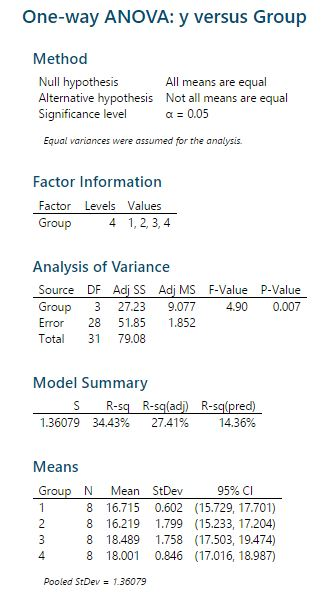
\includegraphics[width=0.8\linewidth]{images/Repeat2017-Output}
\caption{Minitab Out for Q2 Part A}
\label{fig:Repeat2017-Output}
\end{figure}

\newpage
\begin{figure}[h!]
\centering
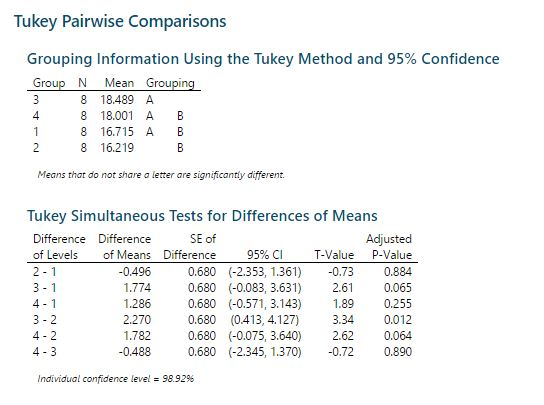
\includegraphics[width=1.1\linewidth]{images/Repeat2017-Output2}
\caption{Minitab Out for Q2 Part A - Continued}
\label{fig:Repeat2017-Output2}
\end{figure}

\begin{figure}[h!]
\centering
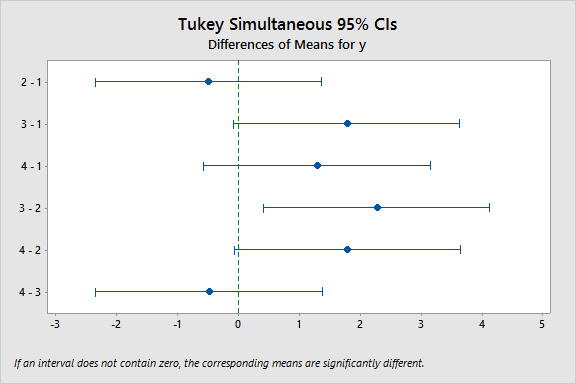
\includegraphics[width=0.6\linewidth]{images/Repeat2017-Q2a-1}
\caption{Post Hoc Tests - Plot 1}
\label{fig:Repeat2017-Q2a-1}
\end{figure}

\newpage
\begin{figure}[h!]
	\centering
	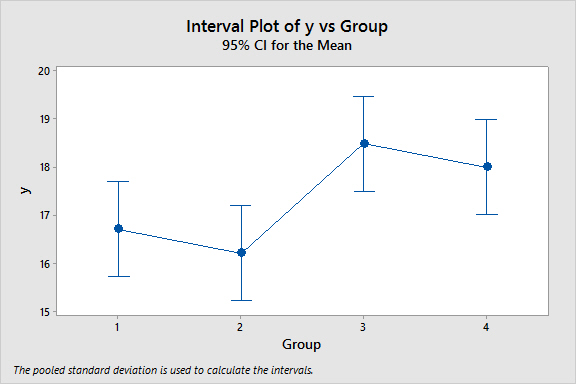
\includegraphics[width=0.7\linewidth]{images/Repeat2017-Q2a-2}
\caption{Post Hoc Tests - Plot 2}
	\label{fig:Repeat2017-Q2a-2}
\end{figure}

\begin{figure}[h!]
	\centering
	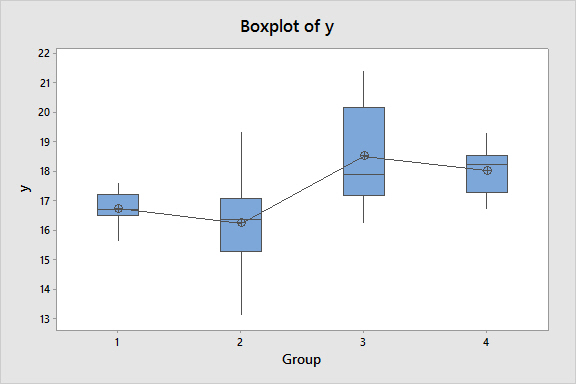
\includegraphics[width=0.7\linewidth]{images/Repeat2017-Q2a-4}
\caption{Post Hoc Tests - Plot 3}
	\label{fig:Repeat2017-Q2a-4}
\end{figure}


\newpage
\subsubsection*{Part B - Two Way ANOVA (10 Marks)}
	\noindent An experiment is conducted to study how long different digital camera batteries last. The 	aim is to find out whether there is a difference in terms of battery life between four brands of 
	batteries using 5 different cameras. Each battery was tried 4 times with each camera.   You are also interested in determining if there is an interaction between the two variables.
	
	


\noindent This data was entered into Minitab and the output on this page and the next page was generated. Write a short report about what this analysis says about the relationship between the battery lifetimes and both of the factors. Explain your conclusions.


\begin{figure}[h!]
\centering
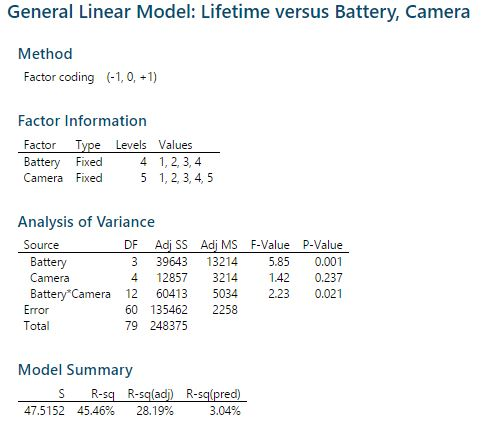
\includegraphics[width=01.1\linewidth]{images/Repeat2017-Q2b-Output1}
\caption{Minitab Output for Question 2 Part B}
\label{fig:Repeat2017-Q2b-Output1}
\end{figure}



\section*{Question 3 - Data Analysis }


%===============================================%

%===============================================%
% Units 3,4 and 5
\subsection*{Part A - Normal Distribution (6 Marks)}

Suppose we have a manufacturing process that is designed to produce a product with a mean weight of 1003 grams. The weight of the products are normally distributed, with a standard deviation of 1.2 grams.


\begin{itemize}
	\item[(a)] (2 Marks) What percentage of products will have a weight exceeding 1005 grams?
	\item[(b)] (2 Marks) What percentage of products will be less than 1000g?
	\item[(c)] (2 Marks) The production manager reports that at least 99\% of the output is between 1000g and 1006g. Do you agree with this statement? Justify your answer with the appropriate calculations.
\end{itemize}

\subsection*{Part B - Testing Distributional Assumptions (8 Marks)}
Consider the results of a statistical analysis carried on both of the sample data sets $X$ and $Y$. These results are presented as Minitab output on subsequent pages.

\begin{itemize}
	\item[(a)] (1 Mark) What sort of analysis are we carrying out? 
	\item[(b)] (1 Mark) What is the relevance of this analysis as part of an overall statistical study.
	\item[(c)] (3 Marks) What is the conclusion of this analysis for the Variable $X$? Justify your answer with reference to 3 separate indications.
	\item[(d)] (3 Marks) What is the conclusion of this analysis for the Variable $Y$? Justify your answer with reference to 3 separate indications.
	
\end{itemize}
\bigskip
\textit{\textbf{Important:} Question 3 comprises a third part: Part C. This part is presented in subsequent pages.}
\newpage
\subsubsection*{Question 3 - Part B - Minitab Output for Variable X}
\begin{figure}[h!]
\centering
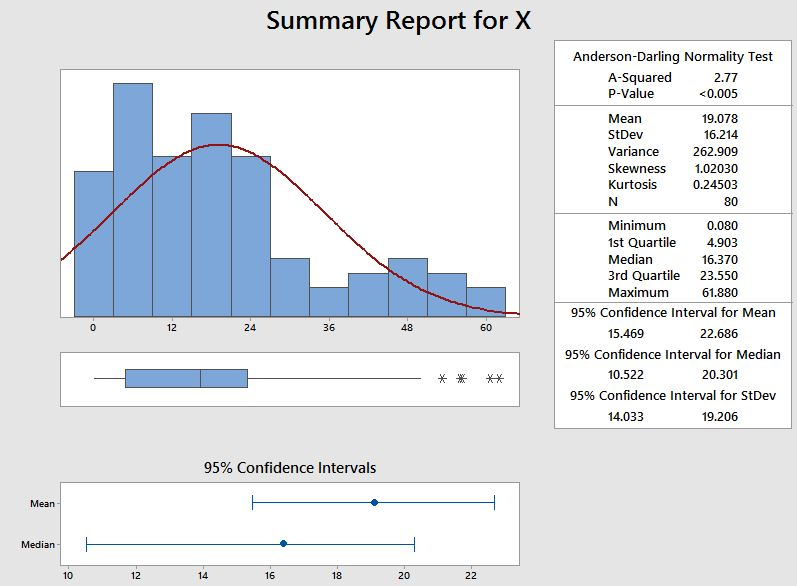
\includegraphics[width=0.99\linewidth]{TestingNormality/NormalityTesting1}
\end{figure}
\begin{figure}[h!]
	\centering
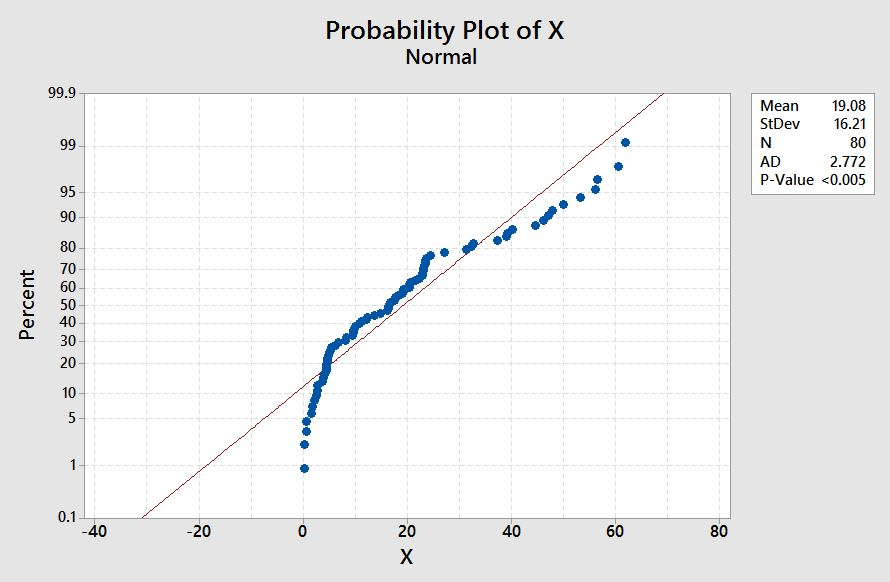
\includegraphics[width=0.99\linewidth]{TestingNormality/NormalityTesting2}
\end{figure}

\newpage
\subsubsection*{Question 3 - Part B - Minitab Output for Variable Y}
\begin{figure}[h!]
	\centering
	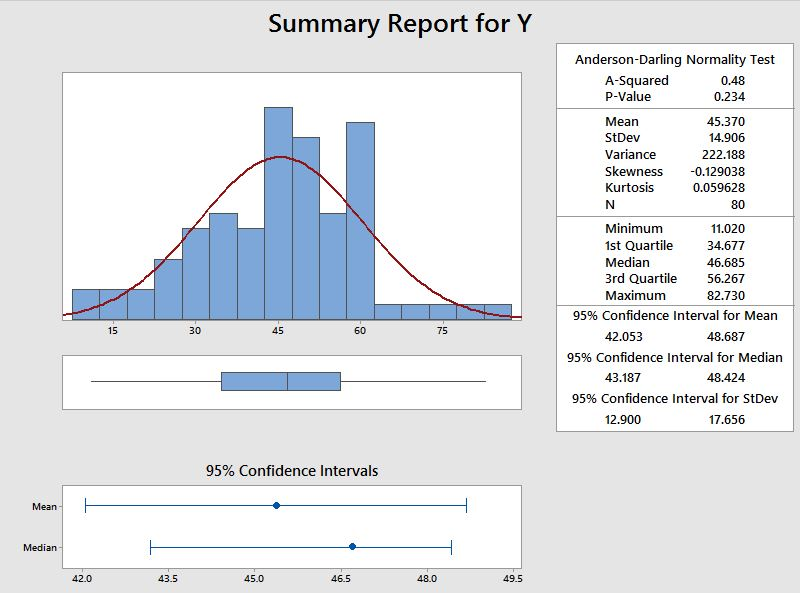
\includegraphics[width=0.99\linewidth]{TestingNormality/NormalityTesting3}
\end{figure}
\begin{figure}[h!]
	\centering
	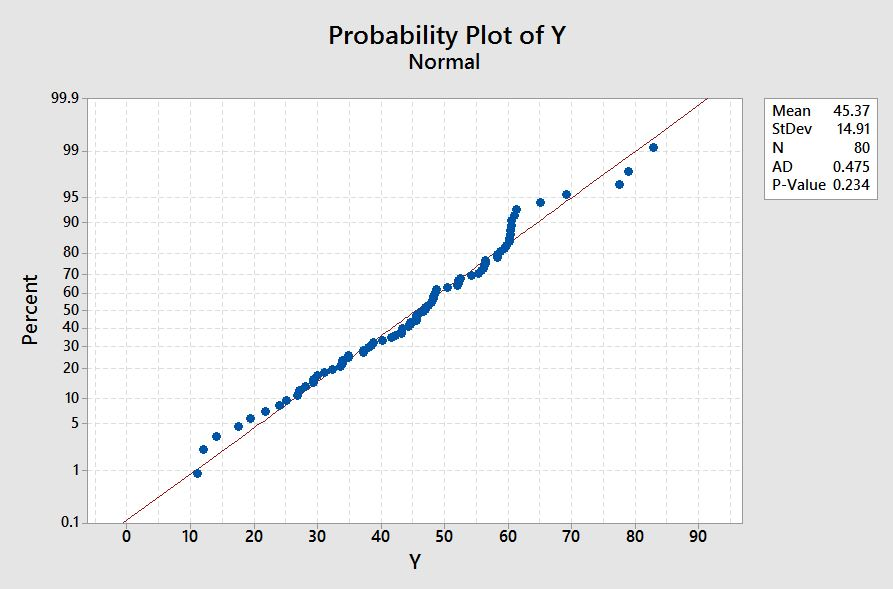
\includegraphics[width=0.99\linewidth]{TestingNormality/NormalityTesting4}
\end{figure}

\newpage


\subsection*{Part C - Boxplots (6 Marks)}
Construct a pair of box plots for the data in the below. Construct one box plot for the data related to Material A, the other for Material B. \\ \medskip \noindent Comment on the features of the box plots and what conclusions, if any, you can derive from the two box plots.
\begin{center}
	\begin{tabular}{|c|c|l|}
		\hline
		Material & Sample size & Bonding Strength (Newton Metres) \\ \hline
		
		A (75\% pure) & 14 & 1.8 2.0 2.1 2.1 2.1 2.2 2.3 2.3 2.3 2.4 2.4 2.5 2.6 2.7 \phantom{sp}
		\\ \hline
		
		B (60\% pure) & 10 & 1.9 1.9 2.0 2.1 2.1 2.2 2.2 2.5 2.7 2.8 \\ \hline
	\end{tabular} 
\end{center}
\medskip
%%\textit{
%%\noindent Marking Scheme:
%%\begin{itemize}
%%	\item 4 Marks for showing the relevant calculations,
%%	\item 1 Mark for drawing the boxplots to a satisfactory standard.
%%	\item 1 Mark for a well-explained conclusion,
%%\end{itemize}
%%}


%====================================================%
\section*{Question 4 - Introduction to Inference}



\subsection*{Part A - Two Sample Mean Test (12 Marks)}
Suppose a company manufactures a particular product in two facilities: Factory A and Factory B.
The management wants to make sure that the Factory B, which has been recently constructed, is manufacturing 
components to the same specifications as Factory A. \\ \smallskip


\noindent Measurement data from both factories has been compiled and analysed, with the following Minitab output has been created.\\ \smallskip

\noindent Using the printout, write a brief report on what the analysis tells you about the comparison of manufacturing processes in both factories. Explain your reasoning clearly. Formally state any null and alternative hypotheses where relevant.
\begin{framed}
\begin{verbatim}
Two-Sample T-Test and CI: Measurement, Factory 

Two-sample T for Measurement

Factory      N     Mean  StDev  SE Mean
FactoryA   240  1002.60   1.76    0.036
FactoryB   260  1002.72   1.64    0.032


Difference = mu (FactoryA) - mu (FactoryB)
Estimate for difference:  -0.1248
95% upper bound for difference:  -0.0456

T-Test of difference = 0 (vs "<0"): 
T-Value = -2.59  P-Value = 0.005  DF = 498
Both use Pooled StDev = 1.7011
\end{verbatim}
\end{framed}

\begin{framed}
\begin{verbatim}
Test and CI for Two Variances: Measurement vs Factory 

Method

Null hypothesis         s(FactoryA) / s(FactoryB) = 1
Alternative hypothesis  s(FactoryA) / s(FactoryB) not equal 1
Significance level      alpha = 0.05


Statistics

95% CI for
Factory      N  StDev  Variance      StDevs
FactoryA   240  1.789     3.202  (1.739, 1.842)
FactoryB   260  1.645     2.705  (1.603, 1.689)

Ratio of standard deviations = 1.088
Ratio of variances = 1.183


95% Confidence Intervals

CI for
CI for StDev      Variance
Method       Ratio           Ratio
Bonett  (1.046, 1.131)  (1.095, 1.279)
Levene  (1.040, 1.130)  (1.082, 1.276)


Tests

Test
Method  DF1   DF2  Statistic  P-Value
Bonett    1   498      14.58    0.000
Levene    1   498      14.58    0.000
\end{verbatim}
\end{framed}
\newpage
\subsubsection*{Question 4 - Part B - Minitab Output for Part A}
\begin{figure}[h!]
\centering
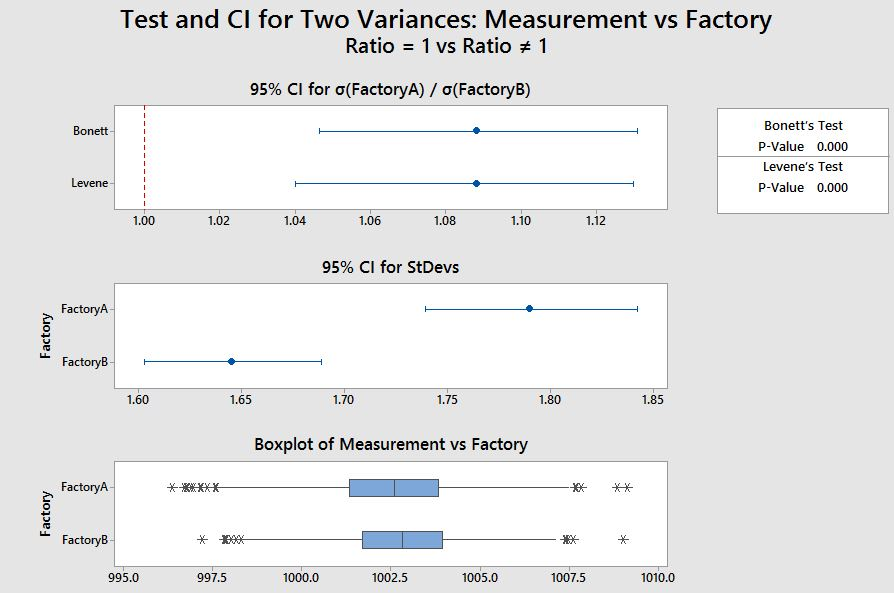
\includegraphics[width=0.9\linewidth]{images/TwoFactoryBoxplots}

\end{figure}


\begin{figure}[h!]
\centering
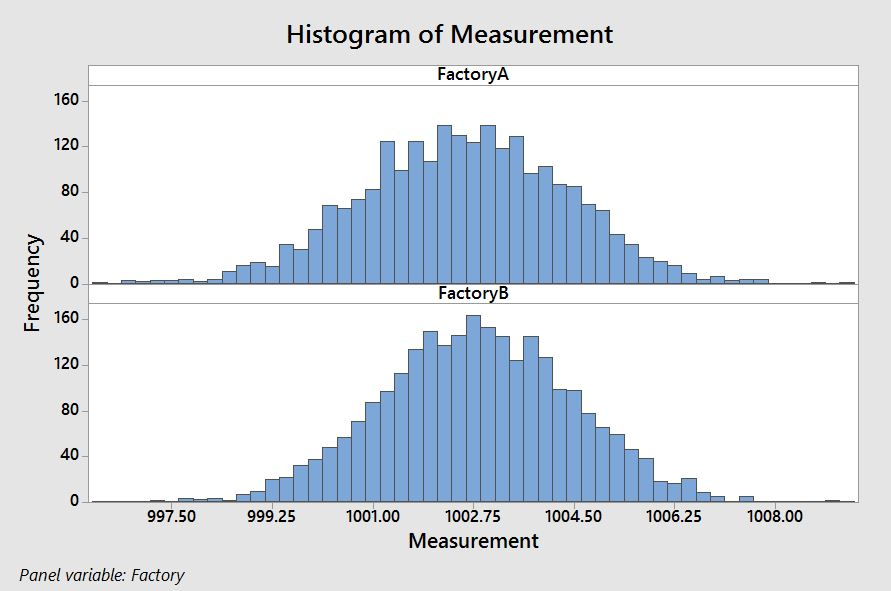
\includegraphics[width=0.9\linewidth]{images/TwoFactoryHistogram}

\end{figure}
\newpage

\subsection*{Part B - Chi Square Tests (8 Marks) }



The research department of an agriculture company are compare the outcomes of pollutant side effects of a fertlizer treatment process on the local water supply. 

\begin{itemize}
	\item There are three research sites. Each of the fertilizer processes is carried out at one of three sites. 
	
	\item There are 100 water quality monitors at each site. The results from each quality monitor is classified as ``None", ``Mild" and ``Severe".
\end{itemize}



\begin{center}
	\begin{tabular}{|c||c|c|c||c|}	
		\hline
		Process &	None	&	Mild	&	Severe	&	Total	\\ \hline
		A	&	30	&	45	&	25	&	100	\\ \hline
		B	&	35	&	45	&	20	&	100	\\ \hline
		C	&	20	&	35	&	45	&	100	\\ \hline
		Total    &	85	&	125	&	90	&	300	\\ \hline
		
	\end{tabular}
\end{center}

The minitab out is tabulated below.
\medskip


%
%
%\bigskip 
%\begin{framed}
%	\noindent \textit{In your answer, you may make reference to the following properties of the Normal Distribution. Consider the random variable $X$ distributed as
%		\[X \sim \mathcal{N}(\mu,\sigma^2)\]
%		where $\mu$ is the mean and $\sigma^2$ is the variance of an random variable $X$.}
%	\begin{itemize}
%		\item $\Pr( \mu - 1\sigma \leq X \leq \mu + 1\sigma ) = 0.6827$
%		\item $\Pr( \mu - 2\sigma \leq X \leq \mu + 2\sigma ) = 0.9545$
%		\item $\Pr( \mu - 3\sigma \leq X \leq \mu + 3\sigma )= 0.9973$
%		
%	\end{itemize}
%\end{framed}

\begin{framed}
	\begin{verbatim}
	Chi-Square Test for Association: C1, Worksheet columns 
	
	Rows: C1   Columns: Worksheet columns
	
	None   Mild  Severe  All
	
	Process A       30     45      25  100
	              ....  .....   .....
	
	Process B       35     45      20  100
	             28.33  41.67   .....
	
	Process C       20     35      45  100
	             .....  .....   30.00
	
	All             85    125      90  300
	
	Cell Contents:      Count
	Expected count
	
	
	Pearson Chi-Square = 17.384, DF = ......., P-Value = 0.002
	Likelihood Ratio Chi-Square = 17.094, DF = ......, P-Value = 0.002
	\end{verbatim}
\end{framed}

\newpage
\begin{itemize}
	\item[(i)] (2 Marks) Provide a brief description of the statistical analysis being carried out here.
	\item[(ii)] (2 Marks) Two expected count values have been removed from the output.
	State what these values should be. Show your workings.
	\item[(iii)] (1 Mark) The ``degrees of freedom" value has been removed from the output. State what the degrees of freedom should be.
	\item[(iv)] (3 Marks) State your conclusions about this procedure. State the null and alternative hypothesis.
	
\end{itemize}






\section*{Question 5 - Regression Models}
\subsection*{Part A - Regression Analysis (8 Marks)}
A wood scientist wishes to determine if there is a relationship between the number of knots in a piece of wood and its tensile strength. A random selection of 16 timber beams were analysed and the results are given in the table below. Following this is a scatter plot of the data.


	
% Sun Oct 09 17:16:35 2016
\begin{table}[ht]
	\centering
\begin{tabular}{|c|c|c|}
	\hline
	Sample &  Number of & Tensile Strength  \\
    number    &   knots  &  N.MS \\
	 \hline	\hline
		1 & 6 & 1.6\\
		2 & 18 & 9.1\\
		3 & 15 & 8.0\\
		4 & 13 & 6.0\\
		5 & 4 & 2.4\\
		6 & 8 & 4.8\\
		7 & 3 & 2.3\\
		8 & 4 & 3.8\\
		9 & 19 & 5.2\\
		10 & 7 & 1.8\\
		11 & 3 & 2.1\\
		12 & 20 & 7.5\\
		13 & 16 & 8.9\\
		14 & 12 & 4.6\\
		15 & 14 & 54  \\
		16 & 9 & 42  \\
		\hline
	\end{tabular}
\end{table}
\textit{(Please turn to the next page for questions.)}
\newpage
\begin{itemize}
	\item[(i)] (2 Marks) Fill in the missing values in the coefficients table of the Minitab printout.
	\item[(ii)] (1 Mark) State the regression equation, as estimated by Minitab.
	\item[(iii)] (3 Marks) Briefly explain what the coefficients table of the Minitab printout tells you about this relationship. 
	\item[(iv)] (1 Mark) Estimate the tensils strength for the case where there is 10 knots on the piece of wood.
 \item[(v)] (1 Mark) How good is this model, in your estimation. Refer to any relevant output in the Minitab printout.
\end{itemize}


\begin{framed}
	\begin{verbatim}
	Model Summary
	
	      S    R-sq  R-sq(adj)  R-sq(pred)
	1.46988  72.40%     70.10%      61.30%
	
	
	Coefficients
	
	Term        Coef  SE Coef  T-Value  P-Value   VIF
	Constant   1.016     1.81     ....    0.606
	Knots      .....   0.0333     6.02    0.000  1.00
	
	
	Regression Equation
	
	...............................
	

	\end{verbatim}
\end{framed}

%\begin{framed}
%	\begin{verbatim}
%	Regression Analysis: Tensile versus Knots 
%	
%	Analysis of Variance
%	
%	Source         DF  Adj SS   Adj MS  F-Value  P-Value
%	Regression      1  68.026  68.0256    31.49    0.000
%	Knots           1  68.026  68.0256    31.49    0.000
%	Error          12  25.927   2.1605
%	Lack-of-Fit    10  24.927   2.4927     4.99    0.179
%	Pure Error      2   1.000   0.5000
%	Total          13  93.952
%	
%	\end{verbatim}
%\end{framed}
\newpage

\subsection*{Part B - Analysis of Residual Plots (4 Marks)}
Minitab can provide four diagnostic plots to help you appraise the quality of a linear model. The diagnostic plots for the regression analysis described in Part A are presented below. \\ \medskip

\noindent What is the purpose of the diagnostic plots and what does each one tell you?

\bigskip

\begin{figure}[h!]
\centering
\includegraphics[width=0.9\linewidth]{"images/Residual Plots for Knots"}
\caption{Diagnostic Plots for Regression Model in Question 5 Part A}
\label{fig:ResidualPlotsforKnots}
\end{figure}




\newpage

\subsection*{Part C - Multiple Linear Regression (8 Marks)}

A logistic companu is researching full efficiency in its fleet of vehicles. The company measured the fuel consumption and 10 aspects of automobile design and performance for 500 vehicles.

\begin{framed}
\noindent The variables are:

\begin{description}
			
			\item[	mpg	]	Miles/(US) gallon
			\item[	cyl	]	Number of cylinders
			\item[	disp	]	Displacement (cu.in.)
			\item[	hp	]	Gross horsepower
			\item[	drat	]	Rear axle ratio
			\item[	wt	]	Weight (1000 lbs)
			\item[	qsec	]	1/4 mile time
			\item[	vs	]	V engine or a straight engine design
			\item[	am	]	Transmission (0 = automatic, 1 = manual)
			\item[	gear	]	Number of forward gears
			\item[	carb	]	Number of carburetors
\end{description}
\end{framed}
\noindent The data was then entered into
Minitab and the following printout was generated.\\
\medskip

\noindent Write a brief report analysing the printout. In your report comment on how well
the model explains the variability in fuel consumption.
Which variable or variables appear to be good predictors of fuel consumption?
Would you refine the model in the light of these results? If so, what changes
would you make?
\newpage
\begin{figure}[h!]
\centering
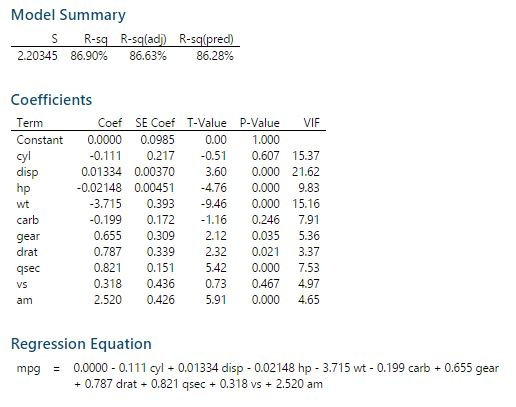
\includegraphics[width=1.1\linewidth]{images/Repeat2017-Q5-Output}
\caption{Minitab Output for Regression Model}
\label{fig:Repeat2017-Q5-Output}
\end{figure}
\newpage
\begin{figure}[h!]
\centering
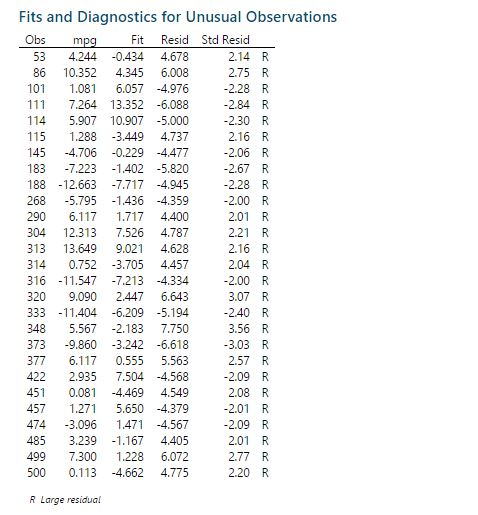
\includegraphics[width=1.1\linewidth]{images/Repeat2017-Q5-Output2}
\caption{Minitab Output for Regression Model - Continued}
\label{fig:Repeat2017-Q5-Output2}
\end{figure}


\end{document}
%============================================================%
\normalsize{


\section*{Formulae}
%-------------------------------------------------%
\subsection*{Descriptive Statistics}
\begin{itemize}
	\item Sample Variance
	\begin{equation*}
		s^2 = \frac{\sum (x-\bar{x})^2}{n-1}
	\end{equation*}
\end{itemize}


\subsection*{Confidence Intervals}
{\bf One sample}
\begin{eqnarray*} S.E.(\bar{X})&=&\frac{\sigma}{\sqrt{n}}.\\\\
	S.E.(\hat{P})&=&\sqrt{\frac{\hat{p}\times(100-\hat{p})}{n}}.\\
\end{eqnarray*}
{\bf Two samples}
\begin{eqnarray*}
	S.E.(\bar{X}_1-\bar{X}_2)&=&\sqrt{\frac{\sigma^2_1}{n_1}+\frac{\sigma_2^2}{n_2}}.\\\\
	S.E.(\hat{P_1}-\hat{P_2})&=&\sqrt{\frac{\hat{p}_1\times(100-\hat{p}_1)}{n_1}+\frac{\hat{p}_2\times(100-\hat{p}_2)}{n_2}}.\\\\
\end{eqnarray*}
%%\subsection*{Hypothesis tests}
%%{\bf One sample}
%%\begin{eqnarray*}
%%	S.E.(\bar{X})&=&\frac{\sigma}{\sqrt{n}}.\\\\
%%	S.E.(\pi)&=&\sqrt{\frac{\pi\times(100-\pi)}{n}}
%%\end{eqnarray*}
%%
%%


\end{document}


\section{Standby}


\subsubsection*{Question 1}


\begin{verbatim}


k) Distinguish between Correlation and Regression when analysing the
relationship between two variables. 




n) What is Simpson?s paradox? 5 marks

o) For each of the following parametric tests give an alternative non parametric test.

(1) Paired t-test (2) F-test (3) Two sample t test 5 marks
\end{verbatim}


	\subsubsection*{Part A - One Way ANOVA (10 Marks )}
	Specimens of milk from dairies in three different districts are assayed for their concentrations of the radioactive isotope Strontium-90. 
	The results, in picocuries per litre, are as shown in the table below.
	
	{
		
		\begin{center}
			\begin{tabular}{|c|cccccc|c|c|}
				\hline  
				District & &&&&& & mean & variance \\  
				&  &&&&&& $\bar{x}_i$ & $s^2_{i}$ \\  
				\hline \hline
				A	&	7.6	&	8.1	&	8.5	&	8.3	&	7.9	&	8.8
				&	8.2	&	0.184	\\ \hline
				B	&	8.7	&	10.2	&	11.4	&	10.9	&	7.2	&	9.2
				&	9.6	&	2.404	\\ \hline
				C	&	10.3	&	9.9	&	11.5	&	11.6	&	10.6	&	8.5
				&	10.4	&	1.312	\\ \hline \hline
				Overall & &&&&&&	9.4	&	2.022 \\ \hline	
				
			\end{tabular} 
		\end{center}
	}
	\bigskip
	\begin{itemize}
		\item[(i)] (2 Marks) Showing your workings, compute the \textbf{Between Group Sum of Squares} (\textit{SSbetween}).
		\item[(ii)] (2 Marks) Showing your workings, compute the \textbf{Within Group Sum of Squares}\\ (\textit{SSwithin}).
		\item[(iii)] (2 Mark) Showing your workings, compute the \textbf{Total Group Sum of Squares} (\textit{SStotal}).
		\item[(iv)] (1 Mark)Complete the \textbf{Degrees of Freedom} Column for the ANOVA table below.
		\item[(iv)] (1 Mark) Complete the \textbf{Mean Square} Column for the ANOVA table below.
		\item[(iv)] (1 Mark) Complete the \textbf{F} Column (i.e. the column for Test Statistic) for the ANOVA table below.
	\end{itemize}
	\newpage
	

\subsubsection*{Question 4 Part A (25 Marks)}

In an investigation into the extraction of nitrate-nitrogen from air dried soil, three quantitative variables were investigated at two levels. These were the amount of oxidised activated charcoal (A) added to the extracting solution to remove organic interferences, the strength of CaSO4 extracting solution (C), and the time the soil was shaken with the solution (T). The aim of the investigation was to optimise the extraction procedure. The levels of the variables are given here:
\begin{center}
	{
		
		\begin{tabular}{|cc|c|c|}
			\hline	&		&\phantom{sp}	{\LARGE -}\phantom{sp}	&	\phantom{sp} {\LARGE +} \phantom{sp}	\\ \hline
			Activated charcoal (g) 	&	A 	&	0.5	&	1	\\ \hline
			CaSO{4} (\%) 	&	C 	&	0.1	&	0.2	\\ \hline
			Time (minutes) 	&	T 	&	30	&	60	\\ \hline
		\end{tabular} 
	}
\end{center}

%\noindent 	The concentrations of nitrate-nitrogen were determined by ultra-violet spectrophotometry and compared with concentrations determined by a standard technique. 
\noindent The results are given below and are the amounts recovered (expressed as the percentage of known nitrate concentration).
{
	
	\begin{center}
		\begin{tabular}{|c|c|c|ccc|}
			\hline
			\phantom{sp}A\phantom{sp}	&	\phantom{sp}C\phantom{sp}	&\phantom{sp}	T\phantom{sp}	&	& y	&	\\
			\hline
			-1	&	-1	&	-1	&	33.95 & 33.46 & 34.32 \\ \hline
			
			1	&	-1	&	-1	&	33.76 & 33.93 & 33.18 \\ \hline
			
			-1	&	1	&	-1	&	34.32 & 35.05 & 34.75 \\ \hline
			
			1	&	1	&	-1	&	32.90 & 32.89 & 33.25 \\ \hline
			
			-1	&	-1	&	1	&	24.88 & 24.33 & 25.46 \\ \hline
			
			1	&	-1	&	1	&	38.67 & 40.23 & 39.14 \\ \hline
			
			-1	&	1	&	1	&	24.57 & 23.93 & 25.49 \\ \hline						
			1	&	1	&	1	&	39.20 & 40.03 & 38.43 \\ \hline
		\end{tabular}
	\end{center}
}











\newpage


\begin{itemize}
	\item[(i.)] (7 Marks) Calculate the contrasts.
	\item[(ii.)] (3 Marks) Calculate the effects.
	\item[(iii.)] (3 Marks) Calculate the sum of squares for the ANOVA Table.
	\item[(iv.)] (4 Marks) Using the computed sums of squares values, complete the ANOVA table (see the \texttt{R} code below).
	\item[(v.)] (4 Marks) Comment on the tests for significant for the main effects and interactions. State clearly your conclusions.
	\item[(vi.)] (4 Marks) Write down a regression equation that can be used predicting amounts based on the results of this experiment.
\end{itemize}
\begin{center}
	\begin{tabular}{|c|c|c|c|c|l|}\hline
		& DF & Sum Sq & Mean Sq & F value&   Pr($>$F)\\  
		\hline A & $\ldots$ & $\ldots$ & $\ldots$  & $\ldots$ &  7.39e$^{-15}$ ***\\ 
		\hline B & $\ldots$ & $\ldots$ & $\ldots$  & $\ldots$ &  0.960  \\ 
		\hline C &\phantom{m} $\ldots$ \phantom{m}  & $\ldots$ & $\ldots$  & $\ldots$ & 3.92e$^{-06}$ *** \\ 
		\hline A:B & $\ldots$ & $\ldots$ & $\ldots$  & $\ldots$ & 0.257 \\ 
		\hline A:C & $\ldots$ & $\ldots$ & $\ldots$  & $\ldots$ & 6.25e$^{-16}$ *** \\ 
		\hline B:C & $\ldots$ & $\ldots$ & $\ldots$  & $\ldots$ & 0.322  \\                 
		\hline A:B:C & $\ldots$ & $\ldots$ & $\ldots$  & $\ldots$ & 0.203  \\ 
		\hline Residuals & $\ldots$ & $\ldots$ &  & &  \\ \hline
		\hline Total & $\ldots$ & 1172.985 &  & &  \\ 	
		\hline 
	\end{tabular} 
\end{center}


\newpage

%====================================================%
\subsection*{Part B - Two Sample Median Test (4 Marks) }
Using the printout, write a brief report on what the analysis tells you about the two
software development tools and discuss the implications of your conclusions. Explain
your reasoning clearly.

\begin{figure}[h!]
	\centering
	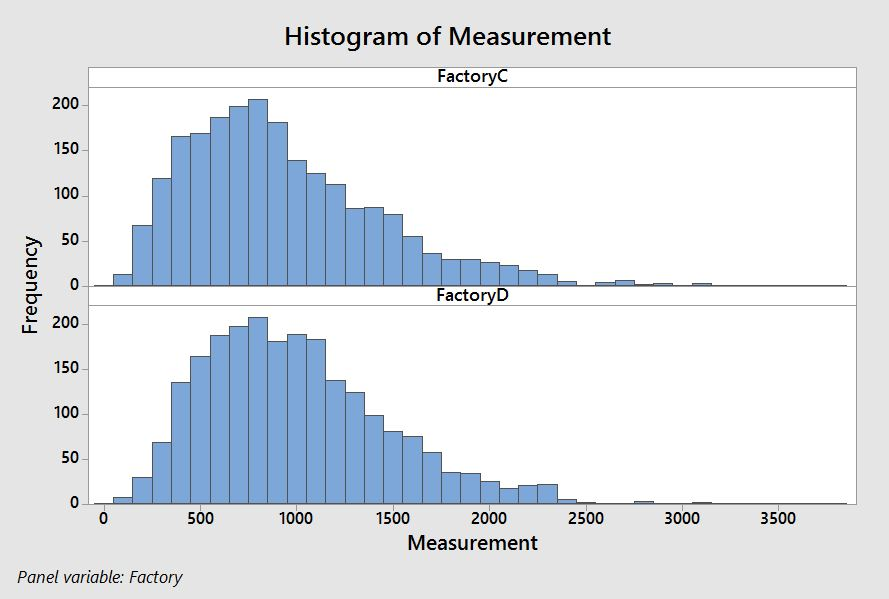
\includegraphics[width=0.9\linewidth]{images/TwoFactoryHistogram-NonParametric}
	\caption{}
	\label{fig:twofactoryhistogram-nonparametric}
\end{figure}
\bigskip
\begin{framed}
	\begin{verbatim}
	
	Mood Median Test: Measurement versus Factory 
	
	Mood median test for Measurement
	Chi-Square = 28.18    DF = 1    P = 0.000
	
	
	\end{verbatim}
\end{framed}
\newpage
\begin{framed}
	\begin{verbatim}
	
	Individual 95.0% CIs
	Factory     N=    N>  Median  Q3-Q1
	FactoryC  1189  1011     837    655 
	FactoryD  1061  1239     931    638 
	
	
	------+---------+---------+---------+
	(----*-----)
	(-------*-----)
	------+---------+---------+---------+
	840       880       920       960
	
	Overall median = 883
	
	
	A 95.0% CI for median(FactoryC) - median(FactoryD): (-128,-57)
	
	
	\end{verbatim}
\end{framed}

\subsection*{Part C (15 Marks)}
% Clincal 

A test of a specific blood factor has been devised such that, for adults in Western Europe, the test score is normally distributed with mean 100 and standard deviation 10. A clinical research organization is carrying out research on the blood factor levels for sufferers of a particular disease.  

\begin{itemize}
	\item A study has obtained the following test scores for 14 randomly selected patients suffering from the disease in Scotland 
	\[ \{118, 116, 114, 110, 118, 111, 124, 117, 107, 116, 125, 93, 
	106, 119\}\]
	
	\item A similar study has obtained the following test scores for 15 randomly selected patients suffering from the disease in Norway.
	\[\{122, 135, 112, 118, 114, 116, 99, 108, 123, 111, 109, 126, 117, 115, 119\}\]
	
\end{itemize}

% The variance of both data sets are equal. 
% You may assume that both data sets are normally distributed.

%===============================%
% 1. outliers
% 3. variance
% 
%===============================%


\newpage
	\subsection*{Question 3 Part C (7 Marks) - The Normal Distribution}
	\noindent A supermarket buys a particular product from five suppliers (V,W,X,Y and Z), and conducts regular tasting tests by three expert panels.
	%are carried out as the product is sold in their food halls. 
	Various characteristics are scored and an analysis of the totals of these scores is made. 
	
	\begin{center}
		\begin{tabular}{|c|c|c|c|c|c|}\hline 
			&	V  & W  & X & Y & Z \\ \hline
			\hline  
			
			Panel 1&   22 &  25 &  23 &  23 &  24 \\ \hline
			Panel 2&   21 &  16 &  16 &  19 &  16 \\ \hline
			Panel 3&   23 &  22 &  19 &  23 &  22 \\ \hline
			
			\hline 
		\end{tabular} 
	\end{center}
	
	\noindent The following questions will result in the completion of the ANOVA Table on the bottom of this page. The $p-$values for both tests are already provided.
	\begin{itemize}
		\item[(i.)](4 Marks) Complete the Sum of Squares column. (Show your workings.)
		\item[(ii.)] (1 Mark) State the degrees of freedom for the ANOVA Table.
		%		\item[(v.)] (1 Marks) Compute the Mean Square values.
		%		\item[(vi.)] (1 Mark) Compute the test statistics for this procedure (i.e. the F-values).
		\item[(iii.)] (2 Marks) Based on the p-values, provided, what is your conclusion? Clearly state the null and alternative hypotheses for both tests.
	\end{itemize}
	
	
	
	%-----------------------------------------------------------------%
	
	

\subsection*{Question 4. (20 marks) Regression Models }


Q4. (a) Discuss the statement ""Correlation does not imply causation"" within the context of data analysis. (4 marks)

%==============================================================%

\begin{itemize}
	
	\item[(i)] Describe the relationship between house size and rebuild cost using the scatter plot below. % (1 mark)
	
	\item[(ii)] Compute the Pearson correlation coefficient. Interpret this value.  %(2 marks)
	
	\item[(iii)] Determine the least squares regression equation. Interpret the meaning of the slope of the regression line. (4 marks)
	
	\item[(iv)] Use the regression line to estimate the rebuild cost for a house sized 120 square metres. %(2 marks)
	
	\item[(v)] Using the 5\% significance level, test the significance of the slope. Interpret the result.  %(6 marks)
	
	\item[(vi)] Calculate and interpret the coefficient of determination.  %(3 marks)
	
	\item[(vi)] What assumptions should a regression model satisfy? How can these assumptions be checked?  %(3 marks)
	
\end{itemize}

\newpage

\subsubsection*{Question 2 Part A (8 Marks)}
In an experiment to determine hydrolysable tannins in plants by absorption spectroscopy, the following results from ten samples were obtained and are tabulated below. A simple linear regression model, predicting absorbance values using concentration as the independent variable, was fitted to the data. The scatterplot is depicted below.
%%Absorbance= c(0.084, 0.183, 0.326, 0.464, 0.643, 0.707, 0.717, 0.734 ,0.749 ,0.732) ;
%%Concentration= c(0.123, 0.288, 0.562, 0.921, 1.420, 1.717, 1.921, 2.137 ,2.321, 2.467) ;
%%plot(Concentration,Absorbance,pch=18,col="red",font.axis=2,font.lab=2)
%%abline(coef(lm(Absorbance~Concentration)))

%%Conc.Squared = (Concentration^2)
%%Conc.Cubed = (Concentration^3)
%%ModelA = lm(Absorbance~Concentration)
%%ModelB = lm(Absorbance~Concentration+Conc.Squared)
%%ModelC = lm(Absorbance~Concentration+Conc.Squared+Conc.Cubed)
\begin{center}
	\begin{tabular}{|c||c|c|c|c|c|}
		\hline
		%  % after \\: \hline or \cline{col1-col2} \cline{col3-col4} ...
		Sample & 1 & 2 & 3 & 4 & 5 \\ \hline
		Absorbance & 0.084& 0.183& 0.326& 0.464& 0.643\\
		Concentration & 0.123& 0.288& 0.562& 0.921& 1.420\\ \hline
		Sample & 6 & 7 & 8 & 9 & 10 \\ \hline
		Absorbance & 0.707& 0.717& 0.734 &0.749 &0.732\\
		Concentration & 1.717& 1.921& 2.137 &2.321&2.467\\
		\hline
	\end{tabular}
\end{center}
%\begin{center}
%	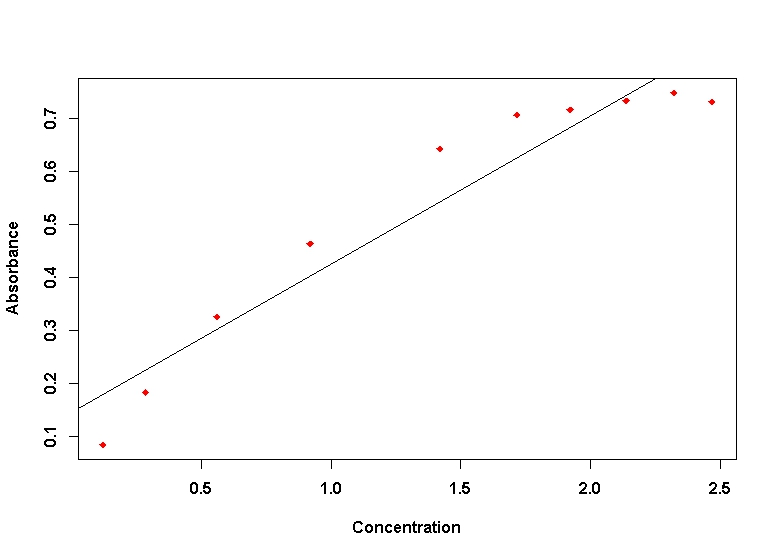
\includegraphics[scale=0.45]{images/ExamQ3plot}
%\end{center}
%\begin{itemize}
%	\item[(i.)] (1 marks) Is the simple linear regression model approach suitable for this study? Explain your answer with reference to the scatter-plot.
%	
%\end{itemize}





